\documentclass[10pt,a4paper]{article}
\usepackage[utf8]{inputenc}
\usepackage[T1]{fontenc}
\usepackage[margin=20mm]{geometry}
\usepackage{amsmath,amssymb}
\usepackage{graphicx}
\usepackage{booktabs}
\usepackage{array}
\usepackage{longtable}
\usepackage[table,dvipsnames]{xcolor}
\usepackage[font=small,labelfont=bf]{caption}
\usepackage{hyperref}
\usepackage{fancyhdr}
\usepackage{enumitem}
\usepackage{float}

\definecolor{hdrblue}{HTML}{2F6FB5}
\definecolor{rowlt}{HTML}{EFF3F8}
\hypersetup{colorlinks=true,linkcolor=hdrblue,urlcolor=hdrblue}
\setlist{itemsep=1pt,topsep=3pt}
\setlength{\parskip}{4pt}
\setlength{\parindent}{0pt}
\newcommand{\hdr}[1]{\textcolor{white}{\textbf{#1}}}
\pagestyle{fancy}
\fancyhf{}
\fancyhead[R]{\small\thepage}
\renewcommand{\headrulewidth}{0.4pt}

\newcommand{\pbtwostartcycle}{114.9}
\newcommand{\pbtwostartviol}{0}
\newcommand{\pbtwostartjoints}{3670.0}
\newcommand{\pbtwostartpath}{7.82}
\newcommand{\pbtwostartmoves}{84}
\newcommand{\pbtwobestcycle}{89.8}
\newcommand{\pbtwobestviol}{0}
\newcommand{\pbtwobestjoints}{2285.0}
\newcommand{\pbtwobestpath}{3.75}
\newcommand{\pbtwobestmoves}{62}
\newcommand{\pbtwobestit}{45}
\newcommand{\pbtwoniter}{53}
\newcommand{\pbtwonkept}{36}
\newcommand{\pbtwonrej}{17}
\newcommand{\pbtwocost}{67}
\newcommand{\pbtwoagentmin}{172}
\newcommand{\pbtwotstart}{2026-11-22 00:16:09}
\newcommand{\pbtwotend}{2026-11-22 03:09:06}
\newcommand{\pbtwonlessons}{48}
\newcommand{\pbtwonagain}{23}
\newcommand{\pbtwofirstlegal}{0}
\newcommand{\pbtwogainpct}{22}

\newcommand{\pbstartcycle}{239.8}
\newcommand{\pbstartviol}{28}
\newcommand{\pbstartjoints}{8911.0}
\newcommand{\pbstartpath}{15.7}
\newcommand{\pbstartmoves}{120}
\newcommand{\pbbestcycle}{112.9}
\newcommand{\pbbestviol}{0}
\newcommand{\pbbestjoints}{3670.0}
\newcommand{\pbbestpath}{7.82}
\newcommand{\pbbestmoves}{84}
\newcommand{\pbbestit}{30}
\newcommand{\pbniter}{30}
\newcommand{\pbnkept}{29}
\newcommand{\pbnrej}{1}
\newcommand{\pbcost}{41}
\newcommand{\pbagentmin}{106}
\newcommand{\pbtstart}{2026-11-20 14:40:34}
\newcommand{\pbtend}{2026-11-20 16:27:52}
\newcommand{\pbnlessons}{30}
\newcommand{\pbnagain}{10}
\newcommand{\pbfirstlegal}{8}
\newcommand{\pbgainpct}{53}

\fancyhead[L]{\small MMA4002 DAM -- Assembly experiment, Part B2 (second blind run, from Part B's best)}

\title{\vspace{-14mm}\textbf{Assembly experiment, Part B2}\\[1mm]
\large A second 3-hour blind run from Part B's best design --- what changed, why, and what it found}
\author{Bjørge (report written by Claude from the run logs)}
\date{Run: \pbtwotstart{} -- \pbtwotend{} on bj-hserver \quad Report: 2026-11-22}

\begin{document}
\maketitle
\thispagestyle{fancy}

\section*{Summary}
%%SUMMARY%%

\section{Why a second run, and what changed in the experiment}
Part B stopped at its 30-iteration cap while it was still improving (iteration 30 was kept), so ``how far can it
go?'' was not answered. B2 continues from Part B's best design. Every change to the experiment, and the reason for it:

\begin{table}[H]
\centering\small
\rowcolors{2}{rowlt}{white}
\begin{tabular}{>{\raggedright}p{40mm} >{\raggedright}p{38mm} >{\raggedright\arraybackslash}p{84mm}}
\toprule
\rowcolor{hdrblue}\hdr{Change} & \hdr{Part B $\to$ B2} & \hdr{Reason}\\
\midrule
Start design & v3 $\to$ Part B's best (iter 30) & Part B ended on its cap, not on a plateau. Starting again from v3 would mostly repeat B.\\
Budget & 30 iterations $\to$ 3\,h wall time & Your request. Late iterations in B took about 3--4\,min each, so a time budget is a fairer limit than a count, and it caps the cost.\\
Stop after no-keep streak & 5 $\to$ 8 & Near the optimum gains are small and rarer; the agent needs more tries before a dead end is real.\\
Judge: Line time & distance only $\to$ max(distance/speed, rotation/50\,deg/s) & Part B's own proposed judge fix (iter 11/30): a real controller limits tool rotation too, and 0\,s re-orientations are a loophole. Baseline re-scored with it (Part B best: 112.9 $\to$ \pbtwostartcycle\,s), so B2 is measured against the same judge.\\
Written reason per change & in the hypothesis $\to$ mandatory \texttt{\#\# Reason} section + \texttt{reason} column & Part B gave its reasons only inside the hypothesis. B2 must name the evidence (a number, a shot, a lesson), the alternatives it rejected and the DFA principle, before it may score. The judge refuses to score without it.\\
Memory & none $\to$ Part B's 30 lessons, 12 standing rules, 25 tools & Tests whether learning carries over between runs, and avoids paying again for the same mistakes.\\
Brief & + ``where run B ended'' & Tells it B's own conclusion (about 70\,\% of the cycle is fixed slow legs and gripper waits), so it looks for structural changes, not only tenths of a second. Risk: this steers it, and the report says so.\\
Kept the same & harness, permissions, hard rules, keep rule, model, speeds & So B and B2 can be compared directly.\\
\bottomrule
\end{tabular}
\caption{Experiment-design changes from Part B to B2.}
\end{table}

\section{Result}
%%RESULT%%

\begin{figure}[H]
\centering
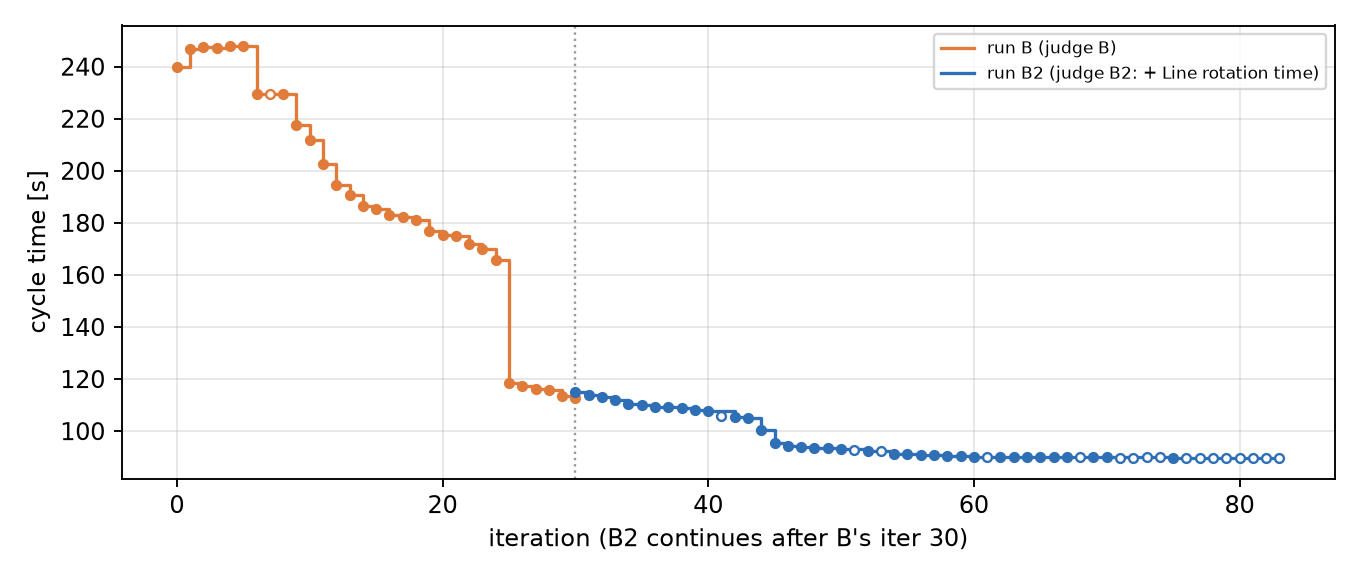
\includegraphics[width=.86\linewidth]{part_b2/fig_combined.png}
\caption{The whole path: run B from v3 (orange, judge B) and run B2 (blue, judge B2, which adds Line rotation time:
+2.0\,s on the same design). Filled = kept, hollow = rejected.}
\end{figure}

\begin{figure}[H]
\centering
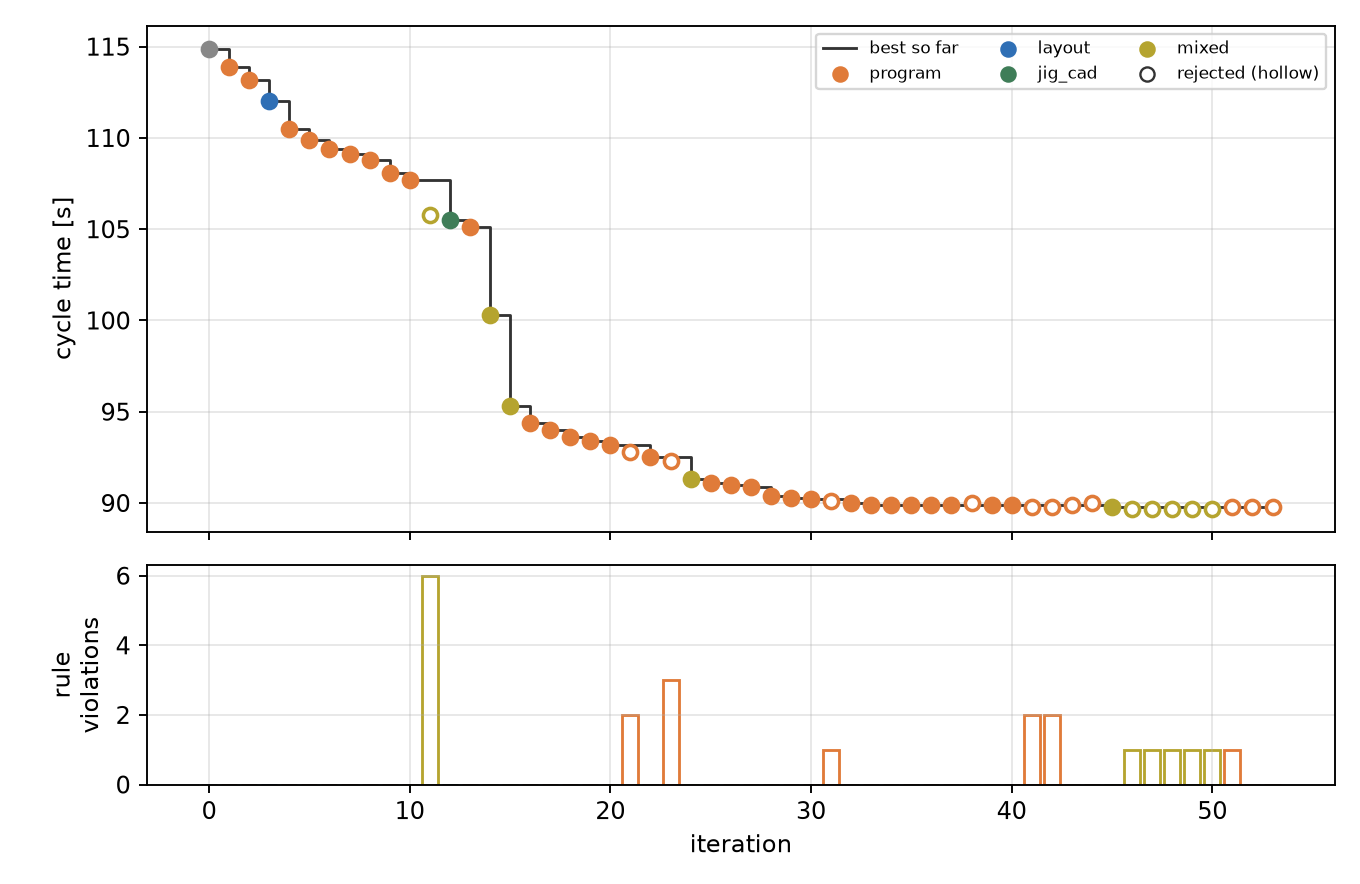
\includegraphics[width=.86\linewidth]{part_b2/fig_progress.png}
\caption{Run B2 alone: every iteration (filled = kept, hollow = rejected, colour = change type) and the best so far.}
\end{figure}

\begin{figure}[H]
\centering
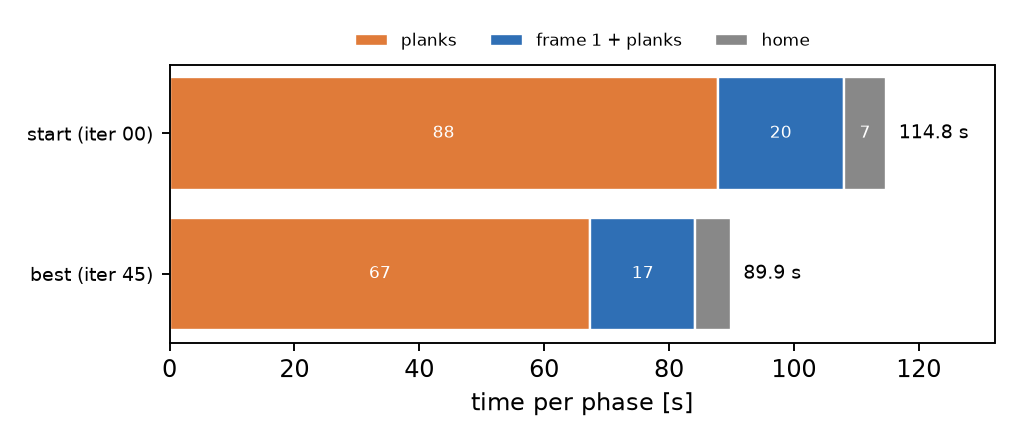
\includegraphics[width=.72\linewidth]{part_b2/fig_phases.png}
\caption{Time per phase, start of B2 vs best of B2.}
\end{figure}

\section{What it changed, and why}
The reason in each row is the agent's own \texttt{Reason} section (first sentences), written before the change was scored.

\begin{figure}[H]
\centering
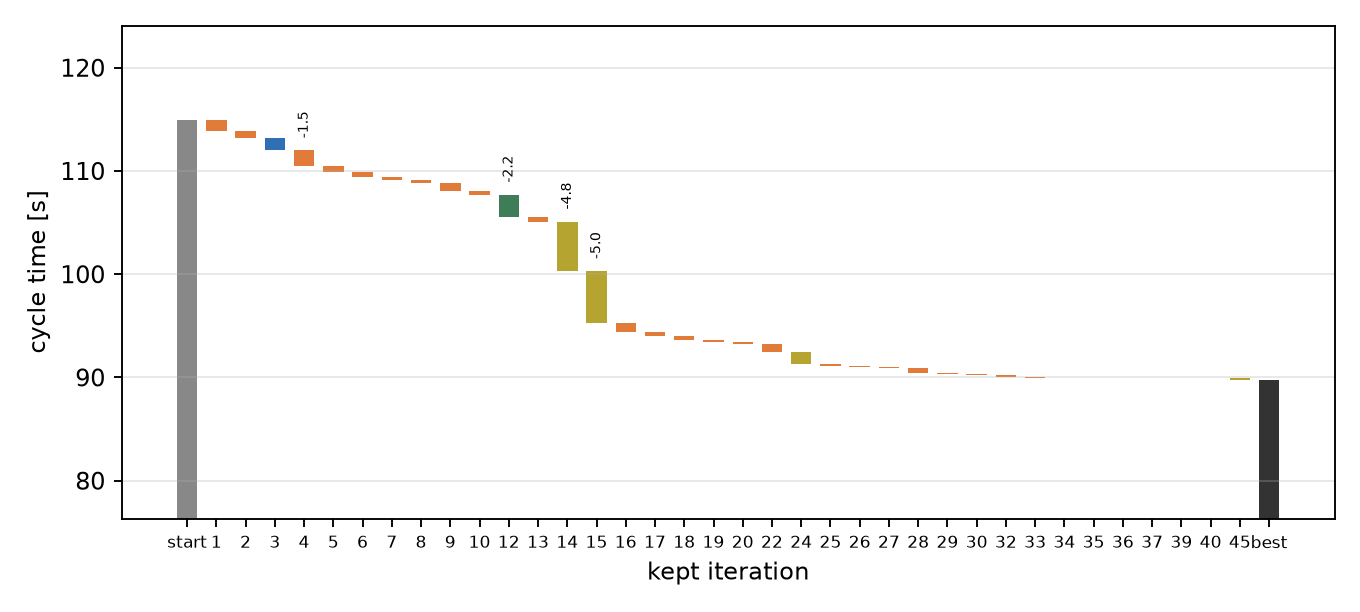
\includegraphics[width=.86\linewidth]{part_b2/fig_waterfall.png}
\caption{Waterfall of B2's kept changes (colour = change type).}
\end{figure}

{\small
\rowcolors{2}{rowlt}{white}
\begin{longtable}{>{\raggedleft}p{5mm} p{12mm} >{\raggedright}p{85mm} r r r p{14mm}}
\toprule
\rowcolor{hdrblue}\hdr{It} & \hdr{Type} & \hdr{Change and reason} & \hdr{Cycle} & \hdr{$\Delta$s} & \hdr{Viol.} & \hdr{Result}\\
\midrule
\endhead
1 & program & \textbf{drop the rotation-limited Line Point65 $\to$ Point70, PTP straight from Point65 to Point80h}\newline Evidence: with the B2 judge (Line time = max(dist/speed, rot/50 deg/s)), toolbox/move\_times2.py shows only two rotation-limited Lines; \#68 Point65 $\to$ Point70 is the bigger one: 39 mm but 76 deg of tool rotation = 1.52 s (was 0.39 s under run B's judge), plus the PTP Point70 $\to$ Point80h 0.78 s. & 113.9 & -1.0 & 0 & kept \\
2 & program & \textbf{pre-rotate the gripper in the fast lift after the plank2 place (\#34), so PTP \#35 turns J6 less}\newline Evidence: toolbox/move\_times2.py on the iter-01 best: PTP \#35 Point38 $\to$ Point25 = 1.52 s, limited by J6 (75.8 deg), the single most expensive plank-phase PTP (others 0.74-1.03 s, J3-limited). & 113.2 & -0.7 & 0 & kept \\
3 & layout & \textbf{move the plank jig 40 mm closer to base A (ground x 250 $\to$ 290) to shorten the J3-limited plank PTPs}\newline Evidence: toolbox/move\_times2.py on the iter-02 best: 11 of the 12 plank-phase PTPs are J3-limited (0.74-1.03 s, $\sim$10.5 s in total); they swing between the pick row at robot x -471..-531 and the base A places at x -653..-748, i.e. a reach change that J3 (elbow) pays for. & 112.0 & -1.2 & 0 & kept \\
4 & program & \textbf{plank transfers as one straight Line between slow-leg tops (drop fast lift + PTP + fast descent)}\newline Evidence: toolbox/move\_times2.py on the iter-03 best: each transfer between two plank events costs fast-up 0.52 + PTP 0.62-0.91 + fast-down 0.52 s = 1.66-1.95 s, 11 transfers $\sim$20 s. & 110.5 & -1.5 & 0 & kept \\
5 & program & \textbf{frame flip as one joint move (drop Point82 / Line Point83 / J5-only Point84)}\newline Evidence: toolbox/move\_times2.py on the iter-04 best: the frame flip Point80L $\to$ Point85 costs 4.46 s, but the J5 change it needs (-53.8 $\to$ +138.1, 192 deg) sets a floor of 3.84 s; the intermediate via points (high Point82, the re-orienting Line, the v3 "J5-only flip" convention) add $\sim$0.6 s above that floor. & 109.9 & -0.6 & 0 & kept \\
6 & program & \textbf{turn the gripper toward the row-2 pick during the slow release leg after plank2}\newline Evidence: toolbox/move\_times2.py on the iter-05 best lists exactly one ROT-LIMITED move: \#26 (d 112.5 mm, rot 80 deg, 1.60 s, 0.475 s over its distance time). & 109.4 & -0.5 & 0 & kept \\
7 & program & \textbf{pre-turn the tool (J6) during the slow release leg after plank4}\newline Evidence: toolbox/move\_times2.py on the iter-06 best: \#58 Point80h 0.99 s "J6" (49.3 deg), and show\_joints gives J4 33.7 deg as its second joint, so $\sim$0.32 s of it is J6 alone. The slow leg \#55 right before it (50.5 mm at 20 mm/s, 2.52 s) turns nothing. Iter 06 proved the same overlap on the plank2 release leg (-0.5 s, clean). & 109.1 & -0.3 & 0 & kept \\
8 & program & \textbf{pre-turn the wrist toward home during the lift after the frame release}\newline Evidence: toolbox/move\_times2.py on the iter-07 best: the home PTP is the single longest move (3.20 s, J5 159.6 deg); the slow leg right before it turns nothing. & 108.8 & -0.3 & 0 & kept \\
9 & program & \textbf{pre-turn the tool from home in the descent to the first plank pick}\newline Evidence: toolbox/move\_times2.py on the iter-08 best: \#2 home $\to$ Point16 1.37 s "J5" 68.4 deg, while the next Line \#3 (0.52 s) and the slow segment \#4 (0.53 s) have rot 0.0. & 108.1 & -0.7 & 0 & kept \\
10 & program & \textbf{pre-turn frame 1 toward the flip during its lift out of base A}\newline Evidence: toolbox/move\_times2.py on the iter-09 best: \#66 Pvia 1.15 s J5 57.6 and \#67 Point85 2.69 s J5 134.3 = 3.84 s, the J5 floor of the flip (L28/L34), while the three lift Lines before it have rot 0.0. & 107.7 & -0.4 & 0 & kept \\
11 & mixed & \textbf{base B toward the robot, frame release on the J5 $<$ 0 wrist branch}\newline Evidence: move\_times2 on the iter-10 best: flip PTPs 0.65 + 2.76 s and home PTP 2.89 s are all J5-limited; L28/L34 say the J5 round trip (-53 $\to$ +138 $\to$ -90, $\sim$420 deg) is the floor at the current release place because the far plate edge has no J5 $<$ 0 solution.\newline \textit{Rejected: Not legal: 6 violations (r1 3, r4 3). The J5$<$0 frame release with base B 250 mm closer cuts the J5 round trip (105.8 s, -1.9 s), but the folded arm (link\_3) hits the carried frame / base B and the fli ...} & 105.8 & -1.9 & 6 & rejected \\
12 & jig\_cad & \textbf{plank jig as one column along base A, slots aligned with the place rows}\newline Evidence: move\_times2 on the iter-10 best: of the 83.2 s plank phase, 66.7 s are fixed (4 slow legs x 2.53 s + 2 waits per plank); the remaining $\sim$16.5 s are transfers, set by the pick-to-place distance: group 1 transfers are 147 mm Lines (1.47 s each) and the return Lines 112-175 mm, group 2 PTPs 0.82-0.91 s (J3, i.e. reach). & 105.5 & -2.2 & 0 & kept \\
13 & program & \textbf{group-2 plank transfers as single Lines (re-test of iter 04's merge after the iter-12 layout)}\newline Evidence: toolbox/move\_times2.py on the iter-12 best: the group-2 transfers still cost 0.52 + 0.68-0.72 + 0.52 = 1.72-1.76 s (plank4 carry 0.52 + 0.33 + 0.35 + 0.52), while after iter 12's column jig their straight distances are only 156-169 mm - below L33's break-even ($\sim$(1.04 s + PTP s) x 100 mm = $\sim$174 mm). & 105.1 & -0.4 & 0 & kept \\
14 & mixed & \textbf{planks 4-6 from a second jig at the plate's far edge (base A + jig 1 move 15 mm toward the robot)}\newline Evidence: toolbox/move\_times2.py on the iter-13 best: the plank phase is 80.6 s, $\sim$66.6 s of it fixed (4 slow legs + 2 waits per plank); the rest is transfers, and the six group-2 transfers (plank6/5/4 carries and returns) are the longest: 1.56-1.69 s, $\sim$9.8 s together, because those planks are placed in frame 1's far column (robo ... & 100.3 & -4.8 & 0 & kept \\
15 & mixed & \textbf{planks 1-3 start in slots cut into base A, right in front of their places (plank jig 1 removed)}\newline Evidence: toolbox/move\_times2.py on the iter-14 best: the group-1 transfers are 1.40 + 1.43 + 1.15 + 1.47 (lift+PTP+ down) + 1.02 s = 6.5 s, set by the $\sim$100-145 mm from plank jig 1 (robot x -560, beside base A) to the y-124 places (x -638..-698). & 95.3 & -5.0 & 0 & kept \\
16 & program & \textbf{place the far column (planks 6, 5, 4) first, then the y-124 row (3, 1, 2)}\newline Evidence: toolbox/move\_times2.py on the iter-15 best: the single largest non-fixed move in the plank phase is \#26, the 163 mm hand-over from the last y-124 place (plank2, robot x -638) to the first jig-2 pick (plank6, x -779): 1.63 s, plus the 1.02 s rotation-limited Line \#24 before it. & 94.4 & -0.9 & 0 & kept \\
17 & program & \textbf{end the frame flip short of its final tilt, finish the turn in the fast descent Line Point86}\newline Evidence: toolbox/move\_times2.py on the iter-16 best: \#55 Point85 2.76 s "J5" 138.1 deg, the largest single movable move left; the next move \#56 is a 52.5 mm fast Line with rot 0.0, i.e. 0.53 s of unused rotation budget ($\sim$26 deg). & 94.0 & -0.4 & 0 & kept \\
18 & program & \textbf{hide more of the start J5 turn in the first slow approach segment (Point26s)}\newline Evidence: toolbox/move\_times2.py on the iter-17 best: \#2 P16s0 0.92 s "J5" 45.8 deg, \#4 Point26s 0.53 s rot 0.0 (26 deg of unused rotation budget), \#3 Point26 0.72 s rot 32.5 (near its 36 deg budget). & 93.6 & -0.4 & 0 & kept \\
19 & program & \textbf{shorter escape Line after the last plank release (Point70y)}\newline Evidence: toolbox/move\_times2.py on the iter-18 best: \#46 Point70y d 113.3 mm, rot 40.1, 1.13 s - the longest movable non-wrist-limited move left in the plank $\to$ frame hand-over; it is distance-limited (rot budget 0.80 s). & 93.4 & -0.2 & 0 & kept \\
20 & program & \textbf{more pre-turn in the fast frame-lift Line (Point80Lt) before the J5-limited flip}\newline Evidence: toolbox/move\_times2.py on the iter-19 best: the frame flip \#54 Pvia (0.66 s, J5 33.2) + \#55 Point85t (2.44 s, J5 122.1) = 3.1 s is the largest movable block left, J5-limited; \#53 has 9 deg of unused rotation budget and \#56 Point86 6.7 deg, but \#56's side is capped by the elbow over the guide (L37/L45, iter 17). & 93.2 & -0.2 & 0 & kept \\
21 & program & \textbf{J5 pre-turn in the slow frame lift (Point81 $\to$ Point80t) to shorten the J5-limited flip}\newline Evidence: toolbox/move\_times2.py on the iter-20 best: Pvia + Point85t = 2.92 s, both J5-limited; Pvia $\to$ Point85t has J4 72.9 / J1 38.5 / J6 38.6 against J5 122.1, so Pvia's J5 can move up $\sim$45 deg before another joint limits.\newline \textit{Rejected: Not legal: r1 2 (frame 1 + planks tilted while still engaged in base A's pocket/slots during the 50 mm lift).} & 92.8 & -0.4 & 2 & rejected \\
22 & program & \textbf{hide more of the home-trip J5 turn in the first pick's slow descent (split Point27's leg)}\newline Evidence: toolbox/move\_times2.py on the iter-20 best: the home trip is \#61 Point1 2.75 s (J5 137.5) + \#2 P16s0t 0.47 s (J5 23.6, J4 19.9 next) = 3.2 s, purely J5-limited (Point88ht J5 +123 $\to$ P16s0t -38; J4 74, J1 46 are far below). & 92.5 & -0.7 & 0 & kept \\
23 & program & \textbf{hide more of the home-trip J5 turn in the last lift Line Point88ht (and slow leg Point88t)}\newline Evidence: toolbox/move\_times2.py on the iter-22 best: \#62 home PTP 2.20 s, J5-limited (110 deg; J4 85 next), while the Line before it, \#61 Point88ht (59.5 mm, 0.59 s), turns only 15.4 of the 29.7 deg its distance pays for.\newline \textit{Rejected: Not legal: r1 3. J5 turn at the lift end Point88ht drops the elbow (link\_3) onto the guide via J1/J2 although J3 is unchanged (L51); elbow-safe orientations cost more Line rotation than they save.} & 92.3 & -0.2 & 3 & rejected \\
24 & mixed & \textbf{planks 4-6 start in slots cut into base A's far wall (plank jig 2 removed)}\newline Evidence: toolbox/move\_times2.py on the iter-22 best: the group-2 transfers (pick top $<$$\to$ place top) cost 0.50 + 0.58 + 0.54 + 0.62 + 0.59 = 2.83 s, set by the $\sim$45-56 mm x gap from plank jig 2 (robot x -778.7, outside base A) to the far-column places (x -733..-722). & 91.3 & -1.2 & 0 & kept \\
25 & program & \textbf{shorten the plank $\to$ frame hand-over Line Point70y (move its rotation into the slow lift, lower its end)}\newline Evidence: toolbox/move\_times2.py on the iter-24 best: \#47 Point70y d 76.8 mm, rot 40.1, 0.80 s "ROT-LIMITED", while \#46 P16eu has 60.1 deg in a 1.675 s slow leg (23 deg unused); Point70y ends at TCP z 385, which was needed when its start/end were inside plank boxes (L29 moved it 30 mm in +y out of them, but kept the height). & 91.1 & -0.2 & 0 & kept \\
26 & program & \textbf{lower the start PTP end P16s0t beside plank6's thin box (shorter first approach Line)}\newline Evidence: toolbox/move\_times2.py on the iter-25 best: \#3 Point26t d 76.5 mm, rot 31.8, 0.77 s - the largest distance-limited fast Line left at a pick; its start height 383 is set by the r4 box rule over plank6, which a sideways offset escapes (L22 used the same 10 mm side-offset trick for the plank transits in run B; L29/L53: re ... & 91.0 & -0.1 & 0 & kept \\
27 & program & \textbf{lower the post-release lift end Point88ht to $\sim$105 mm over the frame release point}\newline Evidence: toolbox/move\_times2.py on the iter-26 best: of the remaining movable moves, \#61 Point88ht 0.59 s is distance- limited with 0.28 s of unused rotation budget, and its 110 mm height over the release point has 10 mm more than r4 needs (L30: end over-long fast Lines at $\sim$105 mm from the nearest grip point). & 90.9 & -0.1 & 0 & kept \\
28 & program & \textbf{shrink the r3 slow-leg margin from 0.5 mm to 0.1 mm (50.5 $\to$ 50.1 mm legs)}\newline Evidence: toolbox/move\_times2.py on the iter-27 best: of 90.9 s, 28 slow legs x 2.53 s = 70.8 s and 7 s of waits are fixed cost; every movable move left is at a rule floor (iter 27: r4 near-point, elbow over the guide, base A / frame1 box at Point80h, J5 limits). & 90.4 & -0.5 & 0 & kept \\
29 & program & \textbf{size the slow-leg float margin to its error (50.1 $\to$ 50.01 mm legs)}\newline Evidence: iter 28 showed the leg margin is our own fixed cost (L57) and 50.1 mm passed r3 everywhere; scratch/exact27.py on the best gives 90.403 s exact, so a -0.126 s change crosses the 0.1 s rounding step (L55). & 90.3 & -0.1 & 0 & kept \\
30 & program & \textbf{lower the plank $\to$ frame hand-over end Point70yt toward its r4 floor (370 $\to$ $\sim$364 mm)}\newline Evidence: toolbox/move\_times2.py on the iter-29 best: \#47 Point70yt d 64.1 mm, rot 20.0 (0.40 s rotation budget), 0.64 s, distance-limited; iter 25 chose z 370 after screening only 370 / 375, while its own notes put the r4 near-point floor at $\sim$360 (L53: re-derive a coordinate from the constraint that binds, not from the last val ... & 90.2 & -0.1 & 0 & kept \\
31 & program & \textbf{slide the frame-approach PTP end Point80h further down its diagonal Line (f $\sim$0.1-0.2)}\newline Evidence: toolbox/move\_times2.py on the iter-30 best: \#49 Point80 d 77.1 mm, rot 0, 0.77 s - the longest distance- limited fast Line left; Point80h sits $\sim$120 mm from Point81 (computed from the TCPs in move\_times2: dx 38.5, dy -30.7, dz 109.3), so it is $\sim$20 mm above its r4 near-point floor.\newline \textit{Rejected: r4 1: lowering Point80h along its Line puts the TCP $<$ 100 mm above Base A (top 41.2, floor 141.2; it was already at 142.5). Only the near-point distance had been checked (L59).} & 90.1 & -0.1 & 1 & rejected \\
32 & program & \textbf{pre-turn the tool in Line \#47 (Point70ytt) toward Point80h so the frame-approach PTP is no longer J4-limited}\newline Evidence: toolbox/move\_times2.py on the iter-30 best: \#47 Point70ytt d 57.4 mm, rot 20.0 deg = 0.574 s distance-limited, i.e. 8.7 deg of unused rotation budget (L30/L36: free rotation in distance-limited Lines), and the next PTP \#48 Point80h is J4-limited (39.1 deg, 0.78 s). & 90.0 & -0.2 & 0 & kept \\
33 & program & \textbf{tighten three remaining PTP/Line end slacks (P16s0tt, Point88htt, Point80h) to cross the 89.95 s rounding step}\newline Evidence: scratch/exact27.py on the iter-32 best gives 89.985 s, 0.035 s above the 89.95 rounding step (L55/L58). & 89.9 & -0.1 & 0 & kept \\
34 & program & \textbf{remove the J2 detour at the flip via point Pvia (tie-break on joint travel)}\newline Evidence: scratch/exact27.py gives 89.940 s exact; the next rounding step (89.85) needs -0.09 s, and iter 33 left every movable move within 1-2 mm of a rule floor. The keep rule breaks cycle ties by joint\_travel\_deg, so a change that keeps cycle at 89.9 and cuts $\ge$ 1 deg of joint travel is a valid "better". & 89.9 & +0.0 & 0 & kept \\
35 & program & \textbf{remove the J3 detour at home (Point1) (tie-break on joint travel)}\newline Evidence: show\_joints on the iter-34 best: through Point88htt $\to$ Point1 $\to$ P16s0tt every joint is monotonic except J3 (-61.9 $\to$ -58.7 $\to$ -60.1), a 2.8 deg back-and-forth; iter 34 noted it as the last detour left after removing Pvia's J2 rise. & 89.9 & +0.0 & 0 & kept \\
36 & program & \textbf{remove the J6 detour around home (Point1 / P16s0tt) (tie-break on joint travel)}\newline Evidence: show\_joints on the iter-35 best: J6 goes 61.9 (Point88htt) $\to$ 26.5 (Point1) $\to$ 17.8 (P16s0tt) $\to$ 66.9 (Point26t) $\to$ 87.2, i.e. $\sim$93 deg of J6 travel where $\sim$25 would do; the PTPs on both sides are J5-limited (110.1 / 20.1 deg), so their J6 deltas are free to shrink. & 89.9 & +0.0 & 0 & kept \\
37 & program & \textbf{home J6 26.5 $\to$ 28 (last J6 detour at home, tie-break on joint travel)}\newline Evidence: show\_joints on the iter-36 best: J6 61.9 (Point88htt) $\to$ 26.5 (Point1) $\to$ 28.0 (P16s0tt) $\to$ 66.9; iter 36 raised P16s0tt to 28 (L61: Line \#3's rotation budget caps it) but left home at 26.5, so home is now 1.5 deg *outside* its neighbours - a 2 x 1.5 deg detour. & 89.9 & +0.0 & 0 & kept \\
38 & program & \textbf{split the start Line \#3 (P16s0tt $\to$ Point26t) at a joint-space midpoint orientation}\newline Evidence: scratch/travel38.py (new: sampled joint travel per move vs |end - start|) on the iter-37 best shows the largest in-move detour in Line \#3: J3 9.3 + J2 2.8 deg extra (the TCP-straight Line with a 31.9 deg tool turn bends the elbow); other detours are 5-6 deg (P16eut J4, Point80Ltt J4).\newline \textit{Rejected: Split of start Line \#3 at a joint-space midpoint: 90.0 s (+0.1, second half rotation-limited: 17.4 deg/50 $>$ 32.5 mm/100) and 2278 deg (+1); the 9 deg J3 bulge is inherent to the TCP-straight rotating ...} & 90.0 & +0.1 & 0 & rejected \\
39 & program & \textbf{J5 pre-turn at P16eut 0.5 deg smaller (J4 bulge in the lift Line, tie-break on joint travel)}\newline Evidence: scratch/travel38.py on the iter-37 best: the second-largest in-move detour is the Line P16ek $\to$ P16eut, J4 5.6 + J3 2.3 deg extra; unlike Line \#3 (L64) its end pose is a free choice (iter-22 style J5 pre-turn), so it can be changed. & 89.9 & +0.0 & 0 & kept \\
40 & program & \textbf{J5 pre-turn at Point80Ltt 0.2 deg (J4 bulge in the frame lift Line, tie-break on joint travel)}\newline Evidence: scratch/travel38.py on the iter-39 best: the largest remaining in-move detour with a free end pose is the Line Point80ut $\to$ Point80Ltt, J4 5.7 deg extra. & 89.9 & +0.0 & 0 & kept \\
41 & program & \textbf{pre-turn J5 at the flip PTP end Point85tt so the Point86 drop Line takes more of the turn}\newline Evidence: toolbox/move\_times2.py on the iter-40 best: \#56 Point85tt PTP 2.44 s J5-limited (122.1 deg), followed by \#57 Point86 Line d 51.0 mm (0.51 s) turning only 19.5 deg, i.e. 6 deg of free rotation budget (L30/L36: free rotation in distance-limited Lines).\newline \textit{Rejected: J5 pre-turn D -6.5 at Point85tt: 89.8 s but r1 2 Guide/link\_3 at \#56/\#57 (elbow drops over the guide, L51/L66); clean smaller turns round to 89.9 s.} & 89.8 & -0.1 & 2 & rejected \\
42 & program & \textbf{iter 41's J5 pre-turn at Point85tt, with the flip end shifted sideways to clear the elbow off the guide}\newline Evidence: iter 41 reached 89.8 s (-0.107 s, the only $\ge$ 0.1 s gain left after L65) but failed on r1 2 "Guide/link\_3" at \#56/\#57; L60 says a collision floor next to a time gain is paid back with a free coordinate, and here the PTP end's xy is free: Point86 is rotation-limited after the turn, so a small sideways offset of Point85t ...\newline \textit{Rejected: J5 pre-turn D -6.5 at Point85tt plus a 4 mm radial shift of its end: 89.8 s but r1 2 Guide/link\_3 at \#56/\#57.} & 89.8 & -0.1 & 2 & rejected \\
43 & program & \textbf{small J5 pre-turn at the flip end Point85tt, sized by a measured link\_3/4-to-guide distance}\newline Evidence: L67 asked for a probe before a third attempt; the new scratch/elbow43.py (min distance link\_3/link\_4 vs Guide per sample) shows the closest point of the flip is the END of PTP \#56 Point85tt, not the Point86 descent: best 5.3 mm there, D -4 (p41a) and D -6.5 (n42a) 0.0 mm.\newline \textit{Rejected: D -1.5 J5 pre-turn at Point85tt: legal (probe: elbow 2.6 mm from guide), 89.924 s exact = 89.9 tie, but joints 2278 vs 2275 (+3): not better.} & 89.9 & +0.0 & 0 & rejected \\
44 & program & \textbf{move 10 \% of the rotation-limited Line \#47 (Point70yttt) into the J2-limited PTP \#48}\newline Evidence: move\_times2 flags \#47 as the only ROT-LIMITED Line in the cycle (29.2 deg in 57.4 mm, 0.584 vs 0.574 s); the next PTP is J2-limited (26.4 deg), so its wrist joints have spare time.\newline \textit{Rejected: 90.0 s vs best 89.9: moving rotation out of the rot-limited Line \#47 slowed the next PTP \#48 (J4/J2 deltas grew) more than the 0.01 s saved.} & 90.0 & +0.1 & 0 & rejected \\
45 & mixed & \textbf{notch the guide's outer corner so iter 41's J5 pre-turn at Point85tt clears link\_3}\newline Evidence: iter 41 scored 89.8 s with exactly one problem, r1 2 "Guide/link\_3" at \#56/\#57; L66-L68 closed the base-B J5 turn for program-only changes. scratch/elbow45.py on the iter-41 program locates the contact: guide point world (-770.8, -187.2, 149) = guide-local (85, -87, 22), i.e. & 89.8 & -0.1 & 0 & kept \\
46 & mixed & \textbf{J5 pre-turn of 6 deg at the high lift end Point88htt (freed by iter 45's guide notch)}\newline Evidence: exact27 shows the home leg is J5-limited (move\_times2 \#62: dJ 110.1 J5, 2.20 s) and the Line before it (\#61, 53.5 mm, 0.53 s) has spare rotation (15.4 of $\sim$26 deg).\newline \textit{Rejected: 89.7 s but r1 1 Guide/link\_3 at \#61 (J5 turn D -6 at Point88htt); a 10 mm edge strip notch was too narrow, the contact moved to its inner wall.} & 89.7 & -0.1 & 1 & rejected \\
47 & mixed & \textbf{iter 46's J5 pre-turn at Point88htt with a deeper guide edge notch (y to -62)}\newline Evidence: iter 46 scored 89.7 s with exactly one problem, r1 1 "Guide/link\_3" at \#61, and the contact moved from the guide's top edge to the 10 mm strip's inner wall (local y -80) - so link\_3 sweeps deeper than 10 mm (L71).\newline \textit{Rejected: 89.7 s but r1 1 Guide/link\_3 at \#61 (J5 turn D -6 at Point88htt); deepening the guide edge notch to y -62 (guessed, no swept-volume probe) did not clear link\_3.} & 89.7 & -0.1 & 1 & rejected \\
48 & mixed & \textbf{iter 46's J5 pre-turn with a guide edge notch sized from a swept-volume probe}\newline Evidence: L72 asked for a swept-volume probe before another cut. scratch/sweep48.py (link\_3/4 vertices inside the guide's local box over all 2 mm samples of \#61) gives x -11.8..57.4, y -90..-46.7, z 20..34.2 - the iter-47 cut missed the whole x $<$ 26 part, which explains why the contact stayed.\newline \textit{Rejected: Guide notch sized from swept-volume probe still leaves r1 Guide/link\_3 at \#61: a slot at y -49.6 caps the cut at y -53, link\_3 reaches -46.7.} & 89.7 & -0.1 & 1 & rejected \\
49 & mixed & \textbf{smaller J5 pre-turn (D -5.5) at Point88htt with iter 48's guide edge notch}\newline Evidence: iter 48 scored 89.7 s with exactly one problem, r1 1 "Guide/link\_3" at \#61, after a cut capped at y -53 by a slot; L73 says size the program change instead. exact27 sweep: D -3 89.783, D -4 89.768 (both round to 89.8 = no gain), D -5.5 89.740 (rounds 89.7 with 0.01 s margin), D -6 89.730 (hits).\newline \textit{Rejected: D -5.5 J5 turn at Point88htt + iter 48 guide notch: 89.7 s but r1 1 Guide/link\_3 at \#61; clean turns (D $\ge$ $\sim$-5) round to 89.8. Base-B J5 turn closed without moving the guide slot.} & 89.7 & -0.1 & 1 & rejected \\
50 & mixed & \textbf{J5 pre-turn D -5.2 at Point88htt with iter 48's guide edge notch}\newline Evidence: L74 asked to measure the clearance at the rounding window's edge before scoring. exact27 puts that edge at D $\sim$ -5.2 (89.745 s, the last value that rounds to 89.7); elbow43 on it shows 0.0 mm through the middle of the Line \#61 (start 17.2, end 1.2 mm).\newline \textit{Rejected: D -5.2 J5 turn at Point88htt + guide notch: 89.7 s but r1 1 Guide/link\_3 at \#61, as elbow43 predicted (0.0 mm). Rounding window and clean range do not overlap; this turn is closed.} & 89.7 & -0.1 & 1 & rejected \\
51 & program & \textbf{J5 pre-turn D -3 at Point88htt (no guide notch)}\newline Evidence: iters 46-50 closed the D $\le$ -5 turn; nobody had probed the smaller, notch-free turns that iter 49 called "clean". elbow43 on D -3 shows 0.0 mm on \#61 samples 11-20 without the notch, so even small turns hit the guide's top edge without iter 48's cut, and the cycle gain (-0.057 s) does not cross a rounding step.\newline \textit{Rejected: J5 turn D -3 at Point88htt: 89.8 s tie, joints +3, r1 1 Guide/link\_3 at \#61 (elbow43 predicted 0.0 mm). Base-B J5 turn closed at every size.} & 89.8 & +0.0 & 1 & rejected \\
52 & program & \textbf{no change - re-score the best (budget end, no live idea)}\newline Evidence: status shows 9 min of budget left and a no-keep streak of 6. toolbox/move\_times2.py on the best (89.8 s): 70 s is slow legs (28 x 2.5 s) and 7 s gripper waits; every movable move is at a floor already measured: Point80h (base A box, L59), Point70yttt / Point86 rot-limited by 0.01 s (L69), Point88htt / Point85tt J5 turn ...\newline \textit{Rejected: No change (budget end): re-score confirms iter 45 best at 89.8 s, 0 violations, 2285 deg; not better. Summary written.} & 89.8 & +0.0 & 0 & rejected \\
53 & program & \textbf{no change - re-score the best (budget end, no live idea)}\newline Evidence: status shows 8 min of budget left and a no-keep streak of 7. As in iter 52 (L77), every movable move is at a measured floor (base-B J5 turn closed by link\_3 vs the guide slot, L66-L76; rot-limited Lines at 0.01 s, L69); the only gains left need a fixed-cost event removed (new plank jig / grip strategy), which does not ...\newline \textit{Rejected: No change (budget end): re-score confirms iter 45 best at 89.8 s, 0 violations, 2285 deg; not better.} & 89.8 & +0.0 & 0 & rejected \\
\bottomrule
\end{longtable}
}


%%PATTERNS%%

\section{What it learnt}
%%LESSONS%%

\section*{Files}
Logs: \texttt{results/part\_b2/log/} (\texttt{iterations.csv} with the \texttt{reason} column,
\texttt{iter\_NN/notes.md}, \texttt{lessons.md}, \texttt{tool\_changes.md}, \texttt{summary.md}); best design:
\texttt{results/part\_b2/best/}; judge: \texttt{judge\_b2/}; runner: \texttt{run\_part\_b2.sh}; figures:
\texttt{report/build\_figs.py part\_b2}.

\end{document}
